\documentclass[11pt]{article}

% personalise page geometry, e.g., margin,
% for your printer and needs
\usepackage[
  a4paper,
  left = 20mm,
  top = 20mm,
  bottom = 15mm,
]{geometry}

% switch off page numbering
\pagenumbering{gobble}

% use for generating tables
\usepackage{csvsimple}
\csvstyle{GSscale}{
  tabular=r|c|c|c|c|c|l,
  table head =
      & 1 & 2 & 3 & 4 & 5 &\\\hline,
  late after line = \\\hline,
  head=false
}
\csvstyle{RSscale}{
  tabular=r|c|c|c|c|c|c|c|, 
  table head = 
      & 1 & 2 & 3 & 4 & 5 & 6 & 7\\\hline, 
  late after line = \\\hline,
  head=false
}

% for circle box
\usepackage{wasysym}

% indents in itemizes
\usepackage{enumitem}

% switch to sans serif
\renewcommand{\familydefault}{\sfdefault}

% factor for table padding
\renewcommand{\arraystretch}{1.6}

% spacing for itemizes
\usepackage{setspace}
\setlength{\parindent}{0cm}
% \doublespacing
\setlist{leftmargin=1.5cm,itemsep=.5\baselineskip,before=\vspace{.5\baselineskip},after=\vspace{\baselineskip}}

% define the robot's name
\def \robot {Care-O-Bot}

% multiple optional arguments in newcommand, loops
\usepackage{xparse}
\usepackage{pgffor}

% handy for open questions
\newcommand{\openquestion}[1]{#1\\[1em]%
\underline{\hspace{14cm}}\\[1.5em]%
\underline{\hspace{14cm}}\\[1.5em]%
\underline{\hspace{14cm}}\\[1.5em]}

\newcounter{scaleCounter}
\newcommand{\createLikertHeader}{


}

% handy for likert-style questions
\NewDocumentCommand{\likertquestion}{ O{Strongly disagree} O{Strongly agree} O{5} m }{%
\setcounter{scaleCounter}{0}
\def\ltablecfg{}
\loop\ifnum\thescaleCounter<#3
  \stepcounter{scaleCounter}
  \edef\ltablecfg{%
    \ltablecfg
    c|
  }%
\repeat

\setcounter{scaleCounter}{0}
\def\lheader{}
\loop\ifnum\thescaleCounter<#3
  \stepcounter{scaleCounter}
  \edef\lheader{%
    \lheader
    \arabic{scaleCounter} &
  }%
\repeat

\setcounter{scaleCounter}{0}
\def\lbullets{}
\loop\ifnum\thescaleCounter<#3
  \stepcounter{scaleCounter}
  \edef\lbullets{%
    \lbullets
    $\ocircle$ &
  }%
\repeat

\begin{center}%
#4\\[1em]%
\begin{tabular}{r|\ltablecfg l}%
 & \lheader \\%
\hline%
#1 & \lbullets #2\\
\hline%
\end{tabular}%
\\[2em]
\end{center}%
}


\setrobot{Example Robot}

\begin{document}

\section*{Kuesioner}
\subsection*{Data Pribadi}

\begin{itemize}
\item[Partisipan\#:]\underline{\hspace{2cm}}
\end{itemize}

Jenis Kelamin:
\begin{multicols}{2}
\begin{itemize}
\item[$\ocircle$] Laki-laki \item [$\ocircle$] Perempuan
\end{itemize}
\end{multicols}

Ras:
\begin{multicols}{3}
\begin{itemize}
\item[$\ocircle$] Bugis
\item[$\ocircle$] Makassar
\item[$\ocircle$] Toraja
\item[$\ocircle$] Duri
\item[$\ocircle$] Lainnya \underline{\hspace{2cm}}
\end{itemize}
\end{multicols}

\begin{itemize}
\item[Tahun lahir:] \underline{\hspace{2cm}} Tahun
\end{itemize}

Pekerjaan:
\begin{multicols}{3}
\begin{itemize}
\item[$\ocircle$] Karyawan
\item[$\ocircle$] Wiraswasta
\item[$\ocircle$] Belum Bekerja
\item[$\ocircle$] Pelajar
\item[$\ocircle$] Pensiun
\end{itemize}
\end{multicols}



\subsection*{Frekuensi akses dan kunjungan tepi laut}


Seberapa sering anda mengunjungi tepi laut?
\begin{multicols}{3}
\begin{itemize}
\item[$\ocircle$] Tiap hari
\item[$\ocircle$] banyak/minggu
\item[$\ocircle$] sekali/minggu
\item[$\ocircle$] sekali/bulan
\item[$\ocircle$] jarang
\end{itemize}
\end{multicols}

Apa kendaraan anda menuju tepi laut?
\begin{multicols}{3}
\begin{itemize}
\item[$\ocircle$] Jalan kaki
\item[$\ocircle$] Sepeda motor
\item[$\ocircle$] Mobil
\item[$\ocircle$] Sepeda
\end{itemize}
\end{multicols}

Berapa lama perjalanan yang anda tempuh untuk ke tepi laut?
\begin{multicols}{3}
\begin{itemize}
\item[$\ocircle$] kurang 5mnt
\item[$\ocircle$] 5mnt-15mnt
\item[$\ocircle$] 15mnt-30mnt
\item[$\ocircle$] 30-60mnt
\end{itemize}
\end{multicols}


Kapan anda mengunjungi tepi laut?
\begin{multicols}{3}
\begin{itemize}
\item[$\ocircle$] Hari apa saja
\item[$\ocircle$] Akhir pekan
\item[$\ocircle$] Hari libur
\end{itemize}
\end{multicols}


Waktu apa anda sering mengunjungi tepi laut?
\begin{multicols}{3}
\begin{itemize}
\item[$\ocircle$] Pagi
\item[$\ocircle$] Siang
\item[$\ocircle$] Sore
\item[$\ocircle$] Kapan saja
\end{itemize}
\end{multicols}

Ruang mana yang anda paling sering kunjungi?
\begin{multicols}{2}
\begin{itemize}
\item[$\ocircle$] A
\item[$\ocircle$] B
\end{itemize}
\end{multicols}


\subsection*{Elemen dan tingkatannya}

\begin{multicols}{2}
Kehadiran jalan paving
\begin{itemize}
\item[$\ocircle$] Semua dipaving
\item[$\ocircle$] Sebagian dipaving
\item[$\ocircle$] Tidak dipaving
\end{itemize}

Pohon dan tanaman
\begin{itemize}
\item[$\ocircle$] Banyak pohon
\item[$\ocircle$] Beberapa pohon
\item[$\ocircle$] Sedikit pohon
\end{itemize}

Fitur air
\begin{itemize}
\item[$\ocircle$] Beberapa fitur air
\item[$\ocircle$] Tidak ada fitur air
\end{itemize}

Fasilitas
\begin{itemize}
\item[$\ocircle$] Toilet
\item[$\ocircle$] Kedai makanan
\item[$\ocircle$] Alat kebugaran
\end{itemize}

Ukuran
\begin{itemize}
\item[$\ocircle$] Luas
\item[$\ocircle$] Sempit
\end{itemize}


Lalu lintas \textit{(Traffic)}
\begin{itemize}
\item[$\ocircle$] Padat
\item[$\ocircle$] Ringan
\end{itemize}

\end{multicols}


Silahkan pilih diantara dua ruang tepi laut dibawah ini yang anda cenderungi?

\begin{itemize}
\begin{figure}[htpb]
    \centering
    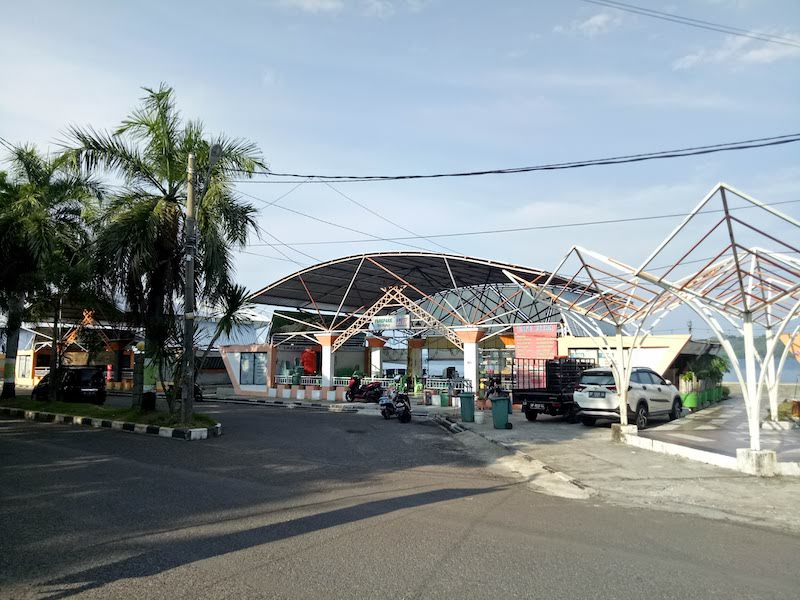
\includegraphics[width=0.65\textwidth]{./figures/ra}
\end{figure}

    \item [$\ocircle$] \qquad Ruang A
\begin{figure}[htpb]
    \centering
    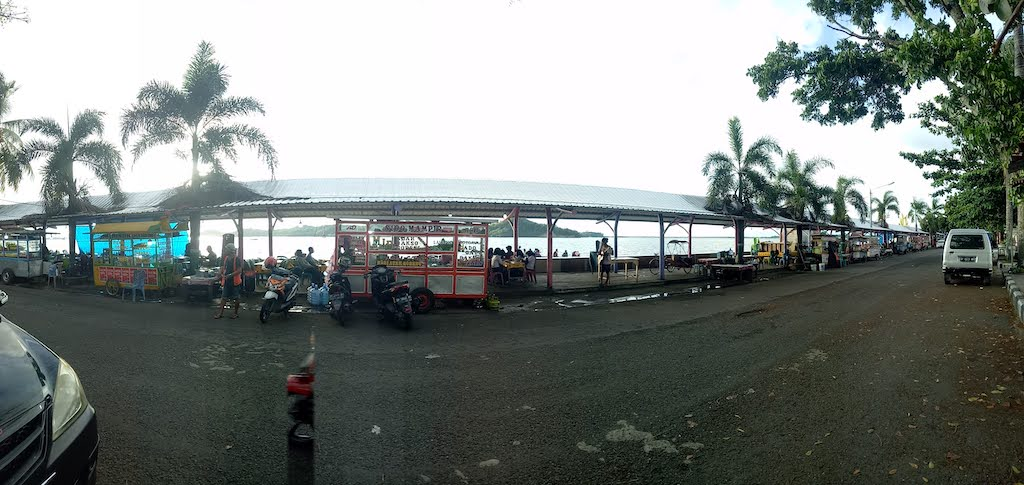
\includegraphics[width=0.65\textwidth]{./figures/rb}
\end{figure}
    \item  [$\ocircle$] \qquad Ruang B
\end{itemize}

Mengapa anda memilih ruang tersebut?


\begin{table}[htpb]
    \centering
    \caption{Set pilihan}
    \label{tab:set}
    \begin{tabular}{p{.23\textwidth} c c p{.23\textwidth}}
    & Ruang A & Ruang B & \centering\arraybackslash Saat ini \\
    Keberadaan paving & Semua dipaving & Sebagian dipaving & \centering\arraybackslash\multirow{6}{*}{\parbox{2cm}{Saya tidak memilih satu pun ruang tersebut}}\\
    Pohon dan tanaman & Banyak pohon & Beberapa pohon & \\
    Fitur air & Beberapa fitur air & Tidak ada fitur air & \\
    Fasilitas & toilet & kedai makanan & \\
    Ukuran & Luas & Sempit & \\
    Lalu lintas & Ringan & Padat & \\

    Saya pilih & $\ocircle$ & $\ocircle$ & \centering{$\ocircle$} \\
    \end{tabular}
\end{table}


\begin{comment}

\subsection*{Pertanyaan 1}
Jika uang, waktu, dan halangan lainnya bukan pertimbangan, ruang mana yang saudara lebih cenderungi untuk dikunjungi? Silakan nilai dengan skala poin 100  dimana ``1" artinya ``kurang dicenderungi" dan ``100" artinya "sangat dicenderungi".

    \begin{tabular}{p{.38\textwidth} c}
    \textbf{Ruang} & \textbf{Nilai kecenderungan}\\
    \end{tabular}
\vspace{10pt}

\score{Ruang A}
\score{Ruang B}

\subsection*{Pertanyaan 2}
Silahkan indikasikan seberapa penting setiap atribut ruang pada ruang publik.

\begin{enumerate}[leftmargin=1em]
    \item \likertquestion[Sangat tidak penting][Sangat penting]{Jarak, kemudahan mengakses jalan dan parkir}
\item \likertquestion[Sangat tidak penting][Sangat penting]{Pencahayaan, keramaian yang terkendali, dan kurangnya gangguan fisik dan sosial}

\item \likertquestion[Sangat tidak penting][Sangat penting]{Keindahan pemandangan}

\item \likertquestion[Sangat tidak penting][Sangat penting]{Keragaman atau ketersediaan penggunaan }
\end{enumerate}

\subsection*{Pertanyaan 3}
\begin{itemize}
    \item Mengapa saudara menyukai ruang tersebut? Deskripsikan dengan detail apa yang menarik menurut saudara tentang atribut ruang itu?

    \item Bagaimana perasaan saudara saat memasuki ruang tersebut?
\end{itemize}
\begin{itemize}
    \item Seberapa sering saudara menggunakan ruang tersebut?
\end{itemize}

\begin{description}
    \item [1] = Belum pernah dengar
    \item [2] = Belum pernah kesana
    \item [3] = Pernah kesana sekali
    \item [4] = Pernah kesana lebih sekali
\end{description}
% Table preferensi ruang
\begin{center}
  \csvreader[ShortScale]{MDRAS/MDRAS-items.csv}{}%
  {\raggedleft \csvcoli & $\ocircle$ & $\ocircle$ & $\ocircle$ & $\ocircle$}%
\end{center}

\subsection*{Pertanyaan 4}
Silakan nilai (centang) pendapat yang paling mewakili pendapat saudara dengan skala poin untuk setiap pernyataan. Dimana ``1" artinya tidak setuju ``5" artinya setuju. \\


Gunakan baris tambahan untuk komentar-komentar.

\begin{enumerate}[leftmargin=1em]
    \item \fivelikert[][]{Jalan setapak membantu menuntun pengunjung ke ruang publik.}
    \openquestion{\,}

    \item \fivelikert[][]{Lahan parkir yang banyak adalah sangat baik untuk setiap orang.}
    \openquestion{\,}

    \item \fivelikert[][]{Tempat yang terbuka memudahkan ruang publik untuk dikenali.}
    \openquestion{\,}

    \item \fivelikert[][]{Ruang publik adalah tempat yang terakses dan inklusif secara sosial dan harus digunakan oleh setiap orang tanpa harus bayar.}
    \openquestion{\,}

%----------------------------------------------------------------------------------------

    \item \fivelikert[][]{Saya kurang enak saat orang lain melihat apa yang saya lakukan.}
    \openquestion{\,}

    \item \fivelikert[][]{Pembatas atau jarak tempat duduk berkontribusi terhadap ruang pribadi (\textit{personal space}) setiap orang}
    \openquestion{\,}

    \item \fivelikert[][]{Vandalisme, sampah, grafiti memberikan kesan negatif ruang publik}
    \openquestion{\,}

    \item \fivelikert[][]{Lampu jalan atau taman dapat memberikan kesempatan untuk berwisata malam}
    \openquestion{\,}

%----------------------------------------------------------------------------------------

    \item \fivelikert[][]{Dapat diterima untuk melepas vegetasi yang ada demi menambahkan pemandangan yang menyorot keindahan alam.}
    \openquestion{\,}


    \item \fivelikert[][]{Warna dan material lantai memberikan gaya pada ruang publik.}
    \openquestion{\,}

    \item \fivelikert[][]{Saya lebih mungkin mengunjungi ruang publik yang bersih dan terpelihara.}
    \openquestion{\,}


%----------------------------------------------------------------------------------------

    \item \fivelikert[][]{Ruang komunal pada ruang publik diinginkan dan membantu interaksi sosial.}
    \openquestion{\,}

    \item \fivelikert[][]{Beberapa aktifitas seperti olahraga, diizinkan di ruang publik (seperti berenang, skateboard \& sepeda).}
    \openquestion{\,}

    \item \fivelikert[][]{Area alami di ruang publik memberikan jalan keluar dari tekanan hidup.}
    \openquestion{\,}

    \item \fivelikert[][]{Ruang gerak yang lebih banyak sangat baik untuk setiap orang.}
    \openquestion{\,}
\end{enumerate}


\section*{Others}
\subsection*{Pertanyaan 2}
%Follow this article Preferences of older people for environmental attributes of local parks- The use of choice‐based conjoint analysis
Silahkan tunjukkan seberapa pentingnya fitur ruang berikut ini ketika mencari tempat di tepi laut.

\likertquestion[Tidak Penting][Penting]{Akses}
\likertquestion[Tidak Penting][Penting]{Fasilitas}
\likertquestion[Tidak Penting][Penting]{Estetika}
\likertquestion[Tidak Penting][Penting]{Keamanan}
\likertquestion[Tidak Penting][Penting]{Pemeliharaan}


\subsection*{Pertanyaan 2}
Silahkan tunjukkan seberapa pentingnya fitur ruang berikut ini ketika mencari tempat di tepi laut.
%% Akses
\likertquestion[Tidak Penting][Sangat Penting]{Lebar sebuah jalan.}
\likertquestion[Tidak Penting][Penting]{Kedekatan fasilitas.}
%% Fasilitas
\likertquestion[Tidak Penting][Penting]{Kehadiran fitur buatan (cth. bangku, lampu jalan).}
\likertquestion[Tidak Penting][Penting]{Kehadiran fitur hijau (cth. tumbuhan, pohon, taman).}
\likertquestion[Tidak Penting][Penting]{Kehadiran fitur biru (cth. kolam, danau, laut).}
%% Estetika
\likertquestion[Tidak Penting][Penting]{Kerapatan vegetasi (tumbuhan, pohon).}
\likertquestion[Tidak Penting][Penting]{Kehadiran tumbuhan (cth. pohon, taman).}
%% Keamanan
\likertquestion[Tidak Penting][Penting]{Ketertutupan sebuah ruang}
\likertquestion[Tidak Penting][Penting]{Keramaian sebuah ruang}
%% Pemeliharaan
\likertquestion[Tidak Penting][Penting]{Kondisi Rumput}
\likertquestion[Tidak Penting][Penting]{Vandalisme}
\likertquestion[Tidak Penting][Penting]{Sampah}

\pagebreak

\subsection*{Pertanyaan 3}
%Silahkan nilai kesan anda terhadap ruang di tepi laut berikut dalam hal "kemudahan akses dengan lebar jalan yang tersedia" dengan skala 7 tingkat dimana "1" mewakili "sangat sulit" dan "7" artinya "sangat mudah".

%Berdasarkan lebar jalan dan kedekatan fasilitas, bagaimana anda menilai ruang di kawasan tepi laut dalam hal "kemudahan atau kesulitanmu untuk mengakses sebuah ruang di kawasan tepi laut" pada skala 7 tingkat dimana "1" mewakili "sangat sulit" dan "7" artinya "sangat mudah".

Berdasarkan lebar jalan dan kedekatan fasilitas, silahkan nilai presepsi anda terhadap ruang-ruang di kawasan tepi laut dalam hal "kemudahan atau kesulitanmu untuk mengakses sebuah ruang di kawasan tepi laut" pada skala 7 tingkat dimana "1" mewakili "sangat sulit" dan "7" artinya "sangat mudah".

    \begin{tabular}{p{.48\textwidth} c}
    & \textbf{Sangat Sulit <-------> Sangat Mudah}
    \end{tabular}

\begin{center}
  \csvreader[LongScale]{MDRAS/MDRAS-items.csv}{}%
  {\raggedleft \csvcoli & $\ocircle$ & $\ocircle$ & $\ocircle$ & $\ocircle$ & $\ocircle$ & $\ocircle$ & $\ocircle$}%
\end{center}


\subsection*{Pertanyaan 4}
Silahkan nilai presepsi anda terhadap ruang-ruang di kawasan tepi laut dalam hal "Ketersediaan fitur buatan (cth. bangku, lampu jalan)" pada skala 7 tingkat dimana "1" mewakili "tidak ada" dan "7" artinya "sangat banyak".


    \begin{tabular}{p{.48\textwidth} c}
    & \textbf{Tidak ada <-------> Sangat Banyak}
    \end{tabular}

\begin{center}
  \csvreader[LongScale]{MDRAS/MDRAS-items.csv}{}%
  {\raggedleft \csvcoli & $\ocircle$ & $\ocircle$ & $\ocircle$ & $\ocircle$ & $\ocircle$ & $\ocircle$ & $\ocircle$}%
\end{center}


\subsection*{Pertanyaan 5}
Silahkan nilai presepsi anda terhadap ruang-ruang di kawasan tepi laut dalam hal "Ketersediaan fitur hijau (cth. pohon, taman)" pada skala 7 tingkat dimana "1" mewakili "tidak ada" dan "7" artinya "sangat banyak".


    \begin{tabular}{p{.48\textwidth} c}
    & \textbf{Tidak ada <-------> Sangat Banyak}
    \end{tabular}

\begin{center}
  \csvreader[LongScale]{MDRAS/MDRAS-items.csv}{}%
  {\raggedleft \csvcoli & $\ocircle$ & $\ocircle$ & $\ocircle$ & $\ocircle$ & $\ocircle$ & $\ocircle$ & $\ocircle$}%
\end{center}


\subsection*{Pertanyaan 6}
Silahkan nilai presepsi anda terhadap ruang-ruang di kawasan tepi laut dalam hal "Ketersediaan fitur hijau (cth. pohon, taman)" pada skala 7 tingkat dimana "1" mewakili "tidak ada" dan "7" artinya "sangat banyak".


    \begin{tabular}{p{.48\textwidth} c}
    & \textbf{Tidak ada <-------> Sangat Banyak}
    \end{tabular}

\begin{center}
  \csvreader[LongScale]{MDRAS/MDRAS-items.csv}{}%
  {\raggedleft \csvcoli & $\ocircle$ & $\ocircle$ & $\ocircle$ & $\ocircle$ & $\ocircle$ & $\ocircle$ & $\ocircle$}%
\end{center}

\subsection*{Pertanyaan 7}
Silahkan nilai presepsi anda terhadap ruang-ruang di kawasan tepi laut dalam hal "Keindahan estetika (termasuk kerapatan vegetasi dan kehadiran tumbuhan)" pada skala 7 tingkat dimana "1" mewakili "sangat polos" dan "7" artinya "sangat indah".


    \begin{tabular}{p{.48\textwidth} c}
    & \textbf{Sangat Polos <-------> Sangat Indah}
    \end{tabular}

\begin{center}
  \csvreader[LongScale]{MDRAS/MDRAS-items.csv}{}%
  {\raggedleft \csvcoli & $\ocircle$ & $\ocircle$ & $\ocircle$ & $\ocircle$ & $\ocircle$ & $\ocircle$ & $\ocircle$}%
\end{center}


\subsection*{Pertanyaan 8}
Berdasarkan tingkat ketertutupan dan keramaian, silahkan nilai presepsi anda terhadap ruang-ruang di kawasan tepi laut dalam hal "rasa aman ketika berada di kawasan tepi laut Senggol" pada skala 7 tingkat dimana "1" mewakili "sangat takut" dan "7" artinya "sangat aman".


    \begin{tabular}{p{.48\textwidth} c}
    & \textbf{Sangat Takut <-------> Sangat Aman}
    \end{tabular}

\begin{center}
  \csvreader[LongScale]{MDRAS/MDRAS-items.csv}{}%
  {\raggedleft \csvcoli & $\ocircle$ & $\ocircle$ & $\ocircle$ & $\ocircle$ & $\ocircle$ & $\ocircle$ & $\ocircle$}%
\end{center}

\subsection*{Pertanyaan 9}

Silahkan nilai presepsi anda terhadap ruang-ruang di kawasan tepi laut dalam hal "pemeliharaan kawasan tepi laut (termasuk keadaan rumput, grafiti dan sampah)" pada skala 7 tingkat dimana "1" mewakili "sangat buruk" dan "7" artinya "sangat baik".


    \begin{tabular}{p{.48\textwidth} c}
    & \textbf{Sangat Takut <-------> Sangat Aman}
    \end{tabular}

\begin{center}
  \csvreader[LongScale]{MDRAS/MDRAS-items.csv}{}%
  {\raggedleft \csvcoli & $\ocircle$ & $\ocircle$ & $\ocircle$ & $\ocircle$ & $\ocircle$ & $\ocircle$ & $\ocircle$}%
\end{center}

\end{comment}
%-------------------------------------------------------------------------------------
% Reference
%-------------------------------------------------------------------------------------

\begin{comment}
% Comments
\subsection*{Comments}
\openquestion{Why did you do XYZ?}\\
\openquestion{Do you have any general impressions about \robot{} during your interaction with it?}\\
\openquestion{Do you have any questions you would like to ask us?}

\pagebreak

% RoSAS

\subsection*{Robot rating}
Using the scale provided, how closely do you associate the following attributes with \robot?%
\begin{center}
  \csvreader[RSscale]{RoSAS/RoSAS-items.csv}{}%
  {\csvcoli & $\ocircle$ & $\ocircle$ & $\ocircle$ & $\ocircle$ & $\ocircle$ & $\ocircle$ & $\ocircle$}%
\end{center}

\pagebreak



% GodSpeed
\subsection*{Robot rating}
Please rate your impression of \robot{} on these scales:%
\begin{center}
  \csvreader[GSscale]{GodSpeed/GodSpeed-items.csv}{}%
  {\csvcoli & $\ocircle$ & $\ocircle$ & $\ocircle$ & $\ocircle$ & $\ocircle$ & \csvcolii}%
\end{center}

\subsection*{Emotional state}
Please rate your own emotional state on these scales:
\begin{center}
  \csvreader[GSscale]{GodSpeed/GodSpeed-items-estate.csv}{}%
  {\csvcoli & $\ocircle$ & $\ocircle$ & $\ocircle$ & $\ocircle$ & $\ocircle$ & \csvcolii}%
\end{center}

\pagebreak


\end{comment}

% MDRAS

\end{document}
